\cleardoublepage
\chapter{Solução}

Neste capítulo iremos explorar a solução encontrada para os vários desafios e necessidades encontradas ao longo desta dissertação.

\section{Autenticação local}

\subsection{Especificação}

De modo a satisfazer as necessidades da autenticação local de utilizadores, através de username e password, foi decidida a implementação de uma base de dados em \emph{MongoDB}.

A criação de um utilizador na plataforma \gls{clav} obriga ao preenchimento dos seguintes dados:

\begin{enumerate}
    \item \textbf{Nome}
    
        Qualquer combinação de números e letras.
    \item \textbf{Email}
    
        Considera-se um email válido qualquer combinação de letras e números, seguida de um "@" com terminação em "." seguido de letras.
    \item \textbf{Nível de utilizador}
    
        Durante a fase de registo é obrigatória a seleção do nível de utilizador do mesmo, sendo esta utilizada para verificação de nível de acesso dentro da plataforma \gls{clav}.
    \begin{enumerate}
        \item Administrador de Perfil Tecnológico
        \item Administrador de Perfil Funcional
        \item Utilizador Validador
        \item Utilizador Avançado
        \item Utilizador Decisor
        \item Utilizador Simples
        \item Representante Entidade
    \end{enumerate}
    \item \textbf{Entidade}
    
        A escolha de uma entidade ao qual o utilizador pertence é de caratér obrigatório, não sendo permitido o registo sem a mesma ser selecionada.
    \item \textbf{Password}
    
        Qualquer combinação de números e letras.
\end{enumerate}

Além da obrigatoriedade dos dados prévios, foi também decidido que todos os dados relativos aos utilizadores iriam ser guardados numa coleção MongoDB com o nome "\emph{users}".

\subsection{Workflow da autenticação}

\begin{figure}[h]
    \centering
    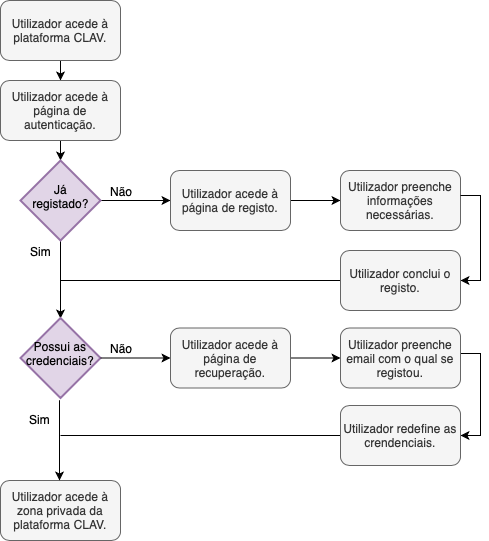
\includegraphics[width=0.75\textwidth]{img/diagramas/authlocal/AuthLocal.png}
    \caption{Workflow da Autenticação local.}
    \label{fig:flow_authlocal}
\end{figure}

\cleardoublepage
\section{Autenticação através de Cartão de Cidadão}
\subsection{Especificação}

A autenticação através de Cartão de Cidadão é baseada na autenticação local, havendo distinção entre os utilizadores registados via username e password, e aqueles registados através de Cartão de Cidadão.

\begin{enumerate}
    \item \textbf{Nome}
    
        Qualquer combinação de números e letras.
    \item \textbf{Email}
    
        Considera-se um email válido qualquer combinação de letras e números, seguida de um "@" com terminação em "." seguido de letras.
    \item \textbf{Nível de utilizador}
    
        Durante a fase de registo é obrigatória a seleção do nível de utilizador do mesmo, sendo esta utilizada para verificação de nível de acesso dentro da plataforma \gls{clav}.
    \begin{enumerate}
        \item Administrador de Perfil Tecnológico
        \item Administrador de Perfil Funcional
        \item Utilizador Validador
        \item Utilizador Avançado
        \item Utilizador Decisor
        \item Utilizador Simples
        \item Representante Entidade
    \end{enumerate}
    \item \textbf{Entidade}
    
        A escolha de uma entidade ao qual o utilizador pertence é de caratér obrigatório, não sendo permitido o registo sem a mesma ser selecionada.
\end{enumerate}

Aquando do registo, a única diferença é que o utilizador registado através de Cartão de CIdadão não possui password, sendo de resto idêntico ao utilizador local.

\cleardoublepage
\subsection{Workflow da autenticação}

\begin{figure}[h!]
    \centering
    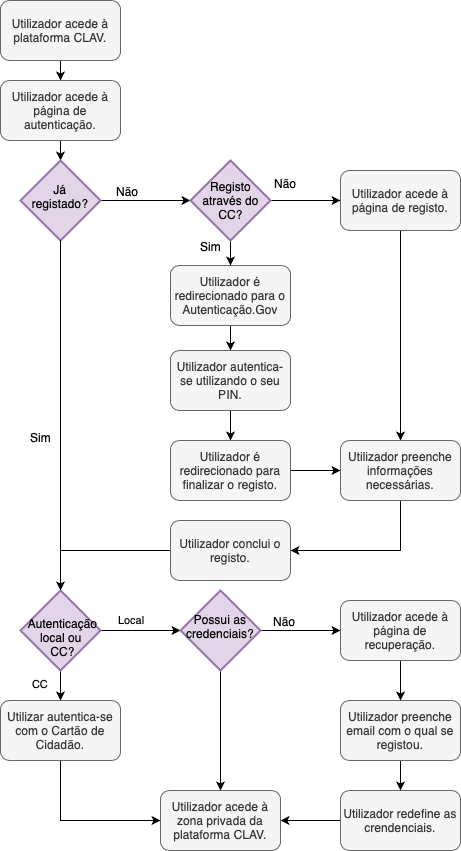
\includegraphics[width=0.695\textwidth]{img/diagramas/authCC/AuthCC.png}
    \caption{Workflow da Autenticação através de Cartão de Cidadão.}
    \label{fig:flow_authCC}
\end{figure}

\cleardoublepage
\section{Proteção da API de dados}

\subsection{Especificação}


\subsection{Workflow da autenticação}